% =====================================================================================
%  Chapter 5 — Discussion
%  Self-contained. Nothing to \input. Requires thesis/references.bib.
%
%  PREAMBLE (already in main.tex): graphicx, booktabs, threeparttable
%  ASSET: figures/fig_stacking.pdf
%    Regenerate:  PYTHONPATH=. python -m experiments.make_fig_stacking
%
%  DEFINES sec:disc:limitations, which Chapters 2 and 3 already reference.
%
%  THE MECHANISM CLAIM IN 5.1 WAS CORRECTED AFTER READING SAFE-GIL. An earlier version said
%  "what transfers is correction of the policy's own behaviour, not instruction from outside
%  it". That is FALSE and the literature already falsifies it: SAFE-GIL clones an MPC or PID
%  controller -- foreign, not the learner -- and safety transfers. The operative variable is
%  the STATE DISTRIBUTION the supervision covers. Do not let the stronger phrasing return.
% =====================================================================================

\chapter{Discussion}\label{ch:discussion}

\section{Why Imitation Succeeds Where Scalar-Reward RL Fails}\label{sec:disc:mechanism}

Both approaches attempted in this work aim at the same target --- move the policy toward the
behaviour the shield induces --- and they differ in the signal used to do it.

Scalar-reward reinforcement learning communicates that target through a single number per
trajectory. The policy must infer, from a reward that fell, which of several hundred actions was
responsible. In a flow-matching policy the only lever available for that inference is the sampling
noise: exploration and credit assignment are the same knob. Increasing the noise enough to
distinguish good actions from bad also degrades the actions being evaluated, so the signal that
drives learning is the signal that destabilises it. This is not a tuning difficulty but a
structural one, and Section~\ref{sec:res:channels} brackets it from both sides: the single
configuration that moved the policy's behaviour collapsed it to inaction, with success reaching
zero even in the shielded condition, while every configuration stable enough to preserve the task
left the unshielded collision rate pinned near 1.0 across six rounds. Those are not two tuned
settings with a working point between them; they are the two sides of one knob.

Imitation replaces the scalar with a dense, per-step target. The shield does not report that a
trajectory was unsafe; it reports what should have been done instead, at every control step where
it intervened, in the same action space the policy emits. Credit assignment is therefore not
inferred but given. The learning signal is also on-distribution by construction: the corrected
actions were produced from states the policy itself visited, so the supervision does not require
the policy to be evaluated in regions it never reaches.

There is a sharper control on this point in the literature, and it is the reason the result
reported here is not a foregone conclusion. Guerrier et al.\ train a reinforcement-learning agent
with a CBF filter active throughout training and then remove it, which is superficially the same
protocol used here~\cite{guerrier2025guardrails}. Their agent does not internalise the constraint:
with the filter disabled it collides, and their critic visualisation shows high positive value
\emph{inside} the obstacle, meaning the policy never represented the hazard at all. The shield had
been present for the entire training run.

The difference is what the policy was trained on. Their agent's actions are overridden by the
filter but the learning signal remains a scalar reward; no gradient ever points toward the
corrected action. The method here behaviour-clones the corrected action itself, so the correction
is the target rather than an intervention the policy is merely subjected to. Their result therefore
establishes something this work depends on: exposure to a shield during training does not by itself
transfer safety, and the imitation objective is doing the work. It also disposes of the obvious
deflationary reading of Chapter~\ref{ch:results} --- that any policy trained under a shield would
end up safe. Their curriculum variant, in which the executed action is a blend of filter and policy
with the filter's weight decayed to zero, does internalise both goal-reaching and obstacle
avoidance, which suggests the present result is an instance of something more general rather than a
property of behaviour cloning specifically.

\subsection*{What the Boundary Result Does and Does Not Show}

The measured contrast in Section~\ref{sec:res:source} sharpens this. Cross-policy distillation,
where the targets were dense and per-step but came from a \emph{foreign} expert, failed as
completely as reinforcement learning did. Dense supervision is therefore not sufficient on its own
--- it must also be supervision at states the policy actually reaches.

It is tempting to state this more strongly, as the claim that what transfers is correction of the
policy's own behaviour and never instruction from outside it. That claim would be false, and the
literature already falsifies it. SAFE-GIL trains a behaviour-cloning policy on demonstrations from
an MPC or PID expert --- foreign controllers, not the learner --- and obtains substantially safer
policies than vanilla behaviour cloning~\cite{ciftci2025safegil}. What makes those demonstrations
work is not the teacher's identity but where they are collected: Hamilton--Jacobi reachability
computes the disturbance that most steers the system toward failure, that disturbance is injected
during collection, and the fixed expert is thereby forced to demonstrate recovery from precisely
the states a learner's errors would produce. Their ablation confirms that this targeting is the
active ingredient, since Gaussian noise, uniform noise and DART all fail to reproduce the benefit.

IntervenGen reaches the same place by a different route. It rolls out the \emph{current} policy in
new scene configurations so that the mistakes it records are that policy's genuine failures rather
than replayed ones, detects each mistake on contact, and transforms a \emph{human} recovery segment
onto the state reached~\cite{hoque2024intervengen}. The recovery actions are again foreign to the
policy; only the states are its own. Two methods, with different teachers --- an optimal controller
in one case, a human operator in the other --- and different means of arriving at the failure
states, therefore locate the active ingredient in the same place.

The correct reading of Section~\ref{sec:res:source} is consequently narrower and more useful. The
planner did not fail because it was foreign. It failed because its trajectories were generated from
its own initial conditions and were never conditioned on where $\pi_{0.5}$ goes wrong, so at
matched sampling it covers the states the student reaches substantially less well ---
Figure~\ref{fig:state_coverage}. The shield succeeded because its corrections are applied, by
construction, at states the policy reached on its own. The operative variable is the \emph{state
distribution the supervision covers}, and self-distillation is one way, not the only way, of
guaranteeing that coverage. Its practical advantage over the adversarial route is that no
disturbance model is needed, because the policy visits its own failure states unprompted.

\section{The Cost of Internalised Caution}\label{sec:disc:cost}

Internalised safety is not free, and this work measured its price in two forms.

The first is time. The distilled policy takes 157.3 control steps to complete a task against 138.6
for the base policy, roughly 14\% slower. It takes a more conservative route, and on a benchmark
where speed is not scored, that cost is invisible in the headline metrics. In a production setting
with cycle-time targets it would not be.

\begin{figure}[htbp]
  \centering
  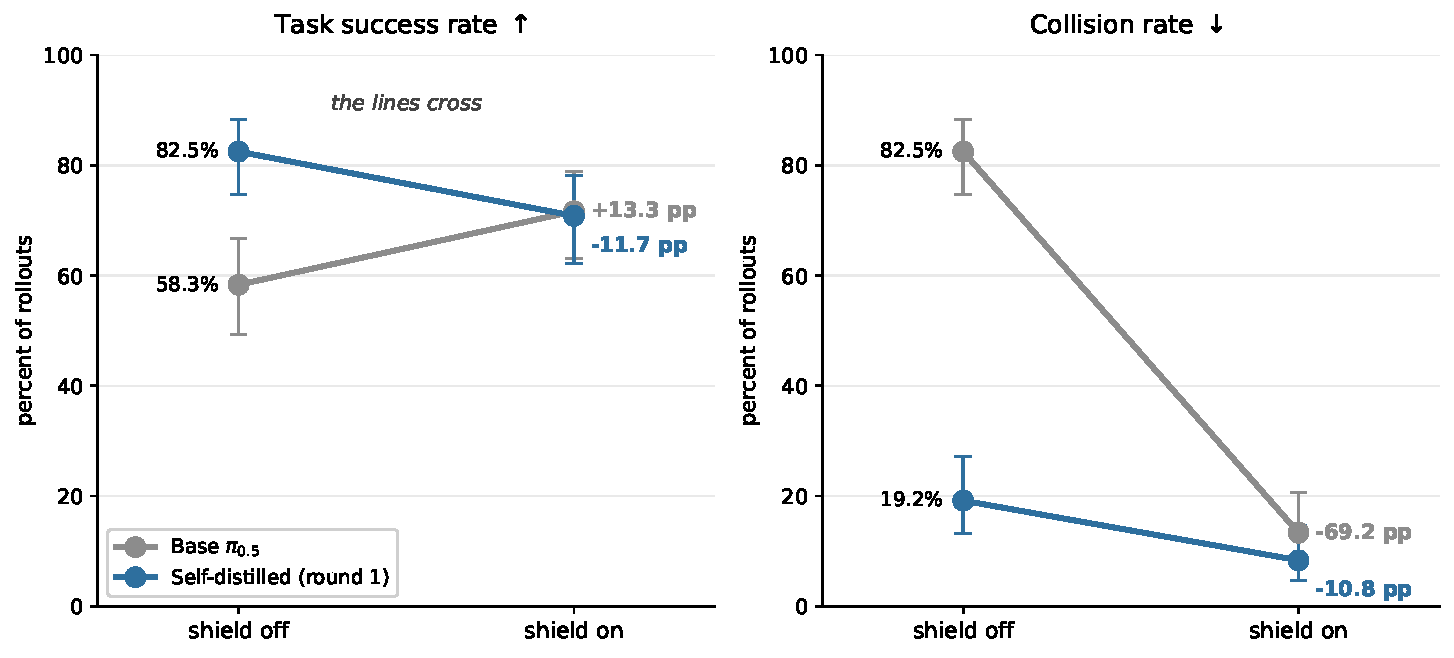
\includegraphics[width=\linewidth]{figures/fig_stacking.pdf}
  \caption[The cost of combining mechanisms]{%
    The same shield helps one policy and harms the other. Attaching it raises the base policy's
    success by 13.3 points and lowers the distilled policy's by 11.7; the lines cross. The reversal
    is confined to the success channel --- collisions fall in both cases --- so safety and
    capability come apart, and only one of them reverses.}
  \label{fig:stacking}
\end{figure}

The second is more interesting, because it is a cost of \emph{combining} mechanisms rather than of
distillation itself. Applying the shield to the already-distilled policy improves safety further
(CAR 80.8\% to 91.7\%) but reduces success from 82.5\% to 70.8\%. The mechanism is visible in how
the shield works: it projects the proposed action onto the safe set, minimising deviation subject
to the barrier constraint. When the policy frequently proposes unsafe actions that projection is a
net benefit --- which is exactly what Section~\ref{sec:shield_efficacy} shows, where the shield
\emph{raises} base success from 58.3\% to 71.7\%. When the policy already avoids the obstacle, the
same projection perturbs actions that were already both safe and competent, displacing them from
the distribution the policy was trained to produce. The result is an action that satisfies the
barrier and no longer executes a well-formed grasp.

This effect is not peculiar to the setup here. The authors of the benchmark report the same
phenomenon independently, observing that enforcing safety with their layer can drive the system
into out-of-distribution states in which the policy may behave erratically and fail to
recover~\cite{vlsa2026}. That an author-acknowledged limitation of runtime shielding is precisely
what distillation removes is, if anything, the clearest argument for internalisation: the distilled
policy is safe without ever being pushed off its own distribution.

Notably, the anticipated cost did not appear. A second distillation round neither improved nor
eroded performance, in contrast to an earlier DAgger-style experiment in this project that degraded
across rounds (Section~\ref{sec:res:source}). One round was sufficient, and iterating was not
harmful.

\section{Limitations}\label{sec:disc:limitations}

\paragraph{Simulation only.}
Every result is from SafeLIBERO. No physical robot was used and no claim of sim-to-real transfer is
made. The two benchmark defects documented in Section~\ref{sec:res:benchmark} are themselves a
reminder that a simulator's measurements are artefacts of its implementation as much as of the
policy under test.

\paragraph{No formal guarantee is inherited.}
The student is no longer protected by the online constraint satisfaction that establishes forward
invariance~\cite{ames2017cbf}, and this work does not establish a replacement. Conditions under
which a learned controller inherits input-to-state safety from a CBF-based expert do
exist~\cite{cosner2022il_cbf}, but they are demanding and none is met here: they require a robust
CBF-QP expert with explicit disturbance margins, where the shield used here is a nominal QP with an
empirically tuned lag buffer; they require known control-affine dynamics, where the plant is a
seven-degree-of-freedom arm under operational-space control with contact; and they require a
CBF-compliancy condition on data density along the safe-set boundary, bounded learning error, and a
known Lipschitz constant, none of which holds for a three-billion-parameter flow-matching policy.
Even when satisfied, the guarantee holds on an expanded safe set that degrades with data sparsity.
What is demonstrated here is an empirical reduction in collisions, and it should be described that
way.

\paragraph{Privileged geometry.}
The barrier is constructed from obstacle poses and meshes read directly from the simulator. A
deployed system would estimate that geometry from perception and inherit the resulting error, so
every shielded figure reported here is an upper bound for this class of filter. The distilled
policy uses no geometry at inference --- a point in favour of internalisation --- but the
dependency remains during \emph{training}.

\paragraph{Approximate robot model.}
The barrier represents the end-effector with three fitted spheres and each arm link with three
point samples carrying a single radius, and infers link velocities through a damped Jacobian
pseudo-inverse rather than optimising them directly (Section~\ref{sec:barrier}).
Section~\ref{sec:res:scope} argues the residual collisions concentrate where that model is
coarsest; that argument is an interpretation of the attribution data, not an independent
measurement of constraint fidelity.

\paragraph{Single training seed.}
Each distilled policy is one training run and seed variance is unquantified. A replication was
attempted but could not be reconciled across compute environments, and is reported rather than
omitted. This is the weakest methodological point in the work.

\paragraph{Single policy and action space.}
One vision-language-action model, one flow-matching action head, one operational-space action
representation. The chunk-level and denoising-time results depend on that architecture and do not
obviously generalise to policies that emit single actions.

\paragraph{Scope of the negative results.}
The reinforcement-learning result is a finding about the reward design and budget tested, not about
safe reinforcement learning as a class; constrained-MDP~\cite{safevla} and world-model
approaches~\cite{safedojo} supply materially richer constraint signals, and the latter is evaluated
on this same benchmark. Similarly, the best-of-$N$ measurement supports a state-dominant account of
collision risk in this policy and benchmark rather than a general claim about generative policies.

\paragraph{Attribution caveats.}
The per-body attribution is a documented lower bound that can miss delayed or indirect contacts,
and the scene-object category is excluded as an artefact rather than interpreted
(Section~\ref{sec:attribution}).

\section{Future Work}\label{sec:disc:future}

The most direct extension is a \textbf{whole-body barrier with a faithful robot model} --- proper
link geometry and directly constrained link velocities rather than a pseudo-inverse estimate.
Section~\ref{sec:res:scope} predicts this would lower the shield's own floor; whether the
improvement then distils is a separate and testable question. It would also make the guided-sampling
negative worth revisiting, since that mechanism was inert only because it inherited the
end-effector scope of the barrier it steered by.

\textbf{Perception-grounded barriers} would remove the privileged-geometry dependency and measure
how much of the reported safety survives estimation error. Learned safety representations offer one
route~\cite{meng2024conbat,sun2025lpb}, though both retain an inference-time correction that this
work is trying to eliminate.

\textbf{Cheaper corrective coverage} is suggested by the scaling argument in
IntervenGen~\cite{hoque2024intervengen}, where corrective data synthesised from ten interventions
outperform a hundred collected directly at a fraction of the cost. The analogous move here is
generating shielded corrective coverage without re-running the shield online for every episode.

\textbf{Dynamic obstacles and human proximity} would test whether the same distillation holds when
the constraint moves, which is the case that matters for the deployment settings this work is
motivated by.

Finally, the boundary result invites a \textbf{mechanism study}. Cross-policy distillation failed;
observation aliasing was measured and rejected as the explanation
(Section~\ref{sec:res:mechanism}), and state coverage is supported but measured only on
end-effector position. Distribution shift and action-distribution mismatch remain as candidates,
and separating them would say something general about when demonstrations transfer between
controllers. A direct comparison against a model-based safe-RL method on this
benchmark~\cite{safedojo} would place the distillation route against the strongest current
alternative.
